\documentclass[11pt]{article}
\usepackage{scicite}
\usepackage[utf8]{inputenc}

% Default packages
\usepackage{amsmath, amsfonts, amssymb, amsthm, epsfig, epstopdf, titling, url, array}
\usepackage{algorithm} 
\usepackage{algorithmic} 
\usepackage{graphicx}
% Because it is convenient
\usepackage{hyperref}

% To insert tables
\usepackage{array}

% We might need some code insertion
\usepackage{minted}

% Also indent first paragraph of a section
\usepackage{indentfirst}


\theoremstyle{plain}
\newtheorem{thm}{Theorem}[section]
\newtheorem{lem}[thm]{Lemma}
\newtheorem{prop}[thm]{Proposition}
\newtheorem*{cor}{Corollary}

\theoremstyle{definition}
\newtheorem{defn}{Definition}[section]
\newtheorem{conj}{Conjecture}[section]
\newtheorem{exmp}{Example}[section]
\newtheorem{pro}{Property}

\theoremstyle{remark}
\newtheorem*{rem}{Remark}
\newtheorem*{note}{Note}



\topmargin 0.0cm
\oddsidemargin 0.2cm
\textwidth 16cm 
\textheight 21cm
\footskip 1.0cm

\newenvironment{sciabstract}{
\begin{quote} \bf}
{\end{quote}}
\renewcommand\refname{References and Notes}

\newcounter{lastnote}
\newenvironment{scilastnote}{\setcounter{lastnote}{\value{enumiv}}
\addtocounter{lastnote}{+1}
\begin{list}
  {\arabic{lastnote}.}
  {\setlength{\leftmargin}{.22in}}
  {\setlength{\labelsep}{.5em}}}
{\end{list}}


% Include your paper's title here

\title{Wikipedia Recommender System with serendipity} 


\author
    {
      Barszezak Yoann, Bricout Rapha\"el, David Nicolas, Dupr\'e R\'emi,\\
      Fouch\'e Aziz, Gourdel Garance, Kaddar Younesse, Mallem Maher,\\
      \\
      \normalsize{Department of Computer science, ENS Paris-Saclay}\\
    }

 

    \date{November 2017}



%%%%%%%%%%%%%%%%% END OF PREAMBLE %%%%%%%%%%%%%%%%



\begin{document} 

% Double-space the manuscript.

\baselineskip10pt

% Make the title.

\maketitle 



% Place your abstract within the special {sciabstract} environment.

\begin{sciabstract}
Abstract: (pas finalisé)\\

Recommendation systems use data treatment techniques in order to do personal recommendations on informations or products. These systems are having a notorious success on the web. However, due to the global increasing amount of information, they are facing a tough challenge : they must be able to produce high-quality recommendations on large scale problems. \\
In this paper we present a client side web-extension for \textit{Wikipedia}. We aim to create and implement a recommender system which could face two problems. For a given user, we would like to propose articles he is likely to be interested in. On the other hand, we also would like to introduce serendipity in order to help the user discovering new subjects he wouldn't have though about, with the help of reinforcement learning.
\end{sciabstract}


\tableofcontents


\section*{Introduction}

Since a few decades, recommender systems have been present almost everywhere ; from audiovisual services like \textit{YouTube} or \textit{Deezer} with the \textit{"Flow"}, to market platforms like \textit{Amazon}, or through apps stores or even web browsers, about everyone uses at least one of them every day. 

Given user previous selections (content streamed, words searched or items bought),they usually consist in algorithms that try to guess which content is likely to be selected by the user next. \\

With statistical learning comes a natural approach to this problem : for each user \textit{John}, the system aims to train a model which tends to fit the user tastes, to be able to deliver good predictions. One of the easiest and most natural way to apply that is to find the users whose tastes are the closest to \textit{John}'s ones. Then, by simply watching at their advice on an asked product, this is easy to get an idea about how it will be likely to be appreciated by \textit{John}.

Unfortunately, there are many limitations in this method. The main one is that, if there are not enough users in the system, and if there are many objects to rate, the intersection between users ratings is the empty set with a high probability. Furthermore, tastes are evolving ; if an user has given a music five stars ten years ago, then there is no reason he still likes it that much. Finally, this approach implies to be able to define a metric on ratable objects, which can sometimes be very difficult, or even poorly relevant. \\

Reinforcement learning with deep neural networks can overcome these drawbacks, by drastically moving the focal. Instead of starting from a state of the system where many users have already given their ratings, it can be beneficial to start from zero for each user, then start building the model depending on his feedbacks. The system gives a new user a first proposition, and according to his advice on this proposition (\textit{I like/I am not interested}, the model proposes him more and more suggestions trying to fit more and more its tastes, trying to get more \textit{I like} which can be seen as the reward of the experience. Of course, the more active the user is the more accurate tends to be the prediction. \\

One of the big questions which has been to be faced has been : To which data set will be applied this theory ? We finally converged to the biggest collaborative encyclopedia all over the world. \\

\textit{Wikipedia} is huge. Only considering English-written articles, there are more than 5,000,000 of pages, describing hundreds of themes. According to official statistics, 600 brand new articles are published each day. In one hand, these values mean a gigantic amount of knowledge within easy reach, but in the other hand the platform gets all the drawbacks of a collaborative system : fake news, vandalism, incomplete articles... 

Even for an experienced user, browsing this mass of data may be hazardous : whereas searching for a precise page works very well, finding new topics connected to subjects the user used to be interested in can be tough. This wanting is called \textit{serendipity}. 

\begin{center}
\textit{"Serendipity means a 'fortunate happenstance' or 'pleasant surprise'." } \textbf{- Wikipedia}
\end{center}

For instance when \textit{A. Fleming}, coming back from its holidays in 1928, found its \textit{staphs} culture boxes contaminated by the mushroom \textit{Penicillium Notatum}, from which he was able to extract an antibiotic substance he called penicillin, it was a kind of serendipity process.

The recommendation model which will be detailed in this paper must take account of this crucial notion : the user has to be grabbed out of his comfort zone, to discover and explore themes he may appreciate.

\section{Problem Overview}

\textbf{Wikipedia}


-Wikipedia\\
-recommander system\\
-serendipity (def)\\
-questions : like/dislike, specific/general\\
-NN\\
-Implementation\\
(at least)

\section{Retrivial of Candidate articles}


\subsection{Distances on articles}

Let's try to understand the idea of proximity between two articles. One way to do it is to introduce a potential function telling us the proximity between two articles.

\subsubsection{Naive Similarity}

Our attempt to define this potential function uses the set of categories linked to an article, it is called the similarity.





\vspace*{5mm}
\begin{defn}
  Let $a_1$ and $a_2$ be two articles. We call $C_1$ (resp. $C_2$) the set of categories linked to $a_1$ (resp. $a_2$).
  We define the similarity of $a_1$ and $a_2$ the following quantity:\\
  \begin{equation*}
    S_C(a_1,a_2) = \frac{Card(C_1 \cap C_2)}{min(Card(C_1),Card(C_2))}
  \end{equation*}
\end{defn}

\begin{rem}
  $\forall a_1\: a_2,\; S_C(a_1,a_2) \in [0,1]$
\end{rem}

\vspace*{5mm}
With this definition in mind, let's seek for an output of the ``Retrivial of Candidate Articles''.


Let's call $a_c$ the current article.
Given an subinterval $I$ of $[0,1]$, one way to find candidate articles will be to pick randomly $N$ articles $(a_i)_{1 \leq i \leq N}$ such that:
\begin{center}
  $\forall i \; S_C(a_c,a_i) \in I$
\end{center}

In this section, we want to pick articles close to the current one. Therefore, we want that $1 \in I$, i.e $I=[b,1]$ where $b$ depends on the number of categories of $a_c$.



\vspace*{5mm}
This approach should work as long as the similarity is precise (in the case of wikipedia, it means as long as an article have a significant number of categories). Unfortunately, some articles are poorly categorised. Moreover, many articles have hidden categories which does not reflects their content. \\
Therefore, an other approach is needed.


\subsubsection{Another distance using word2vect}
The word2vect tool is useful to define distance : because articles are dived into a vectorial space, we can use the traditional tool on them. \\
To compare 2 articles, we assumed that the introduction was quite relevant regarding their similarity. We thus defined the following similarity:
$$S_W(a,a') = 1- \frac{1 - cos(V_a,V_{a'})}{2}= 1-\frac{1-\frac{V_a.V_{a'}}{||V_a||||V_{a'}||}}{2}$$
where : $V_a = \frac{\sum_{\omega\in intro_a}u_\omega f_\omega}{\sum_{\omega\in intro_a}f_\omega}$ and $u_\omega$ is the vector given by word2vect for the word $\omega$ and $f_\omega$ is the frequence of the word $\omega$ in the introduction of $a$.\\
We weight the words depending on their frequence, and then take the sum to associate them a unique vector. This gives a unique vector computed from the introduction of an article $a$.\\
$S_W$ seems to present more details than $S_C$ because in general, notions referring to an article are mentioned in the introduction. 


\subsection{Ontology}
\subsubsection{Construction of the ontology}
Since the distance is given, we have to choice articles to give to \textit{John}. Unfortunately, this model will have troubles with introducing serendipity.\\
A way to solve this problem is to use an Ontology on the wikipedia articles.

\vspace*{5mm}
\begin{defn}
  Let $A$ a set of theme. We call $\mathbb{O}$ an Ontology over $A$ a directed acyclic graph in which :
  \begin{itemize}
  \item $ Node(\mathbb{O}) = A$
  \item if $t_1$ is a direct subtheme of $t_2$ then $(t_1,t_2) \in Edge(\mathbb{O})$
  \end{itemize}
\end{defn}

\vspace*{5mm}

\begin{rem}
  The relation ``is a subtheme'' is not transitive.
\end{rem}
\vspace*{5mm}
\newpage
\begin{exmp}
\end{exmp}
\begin{figure}[!h]
  \center
  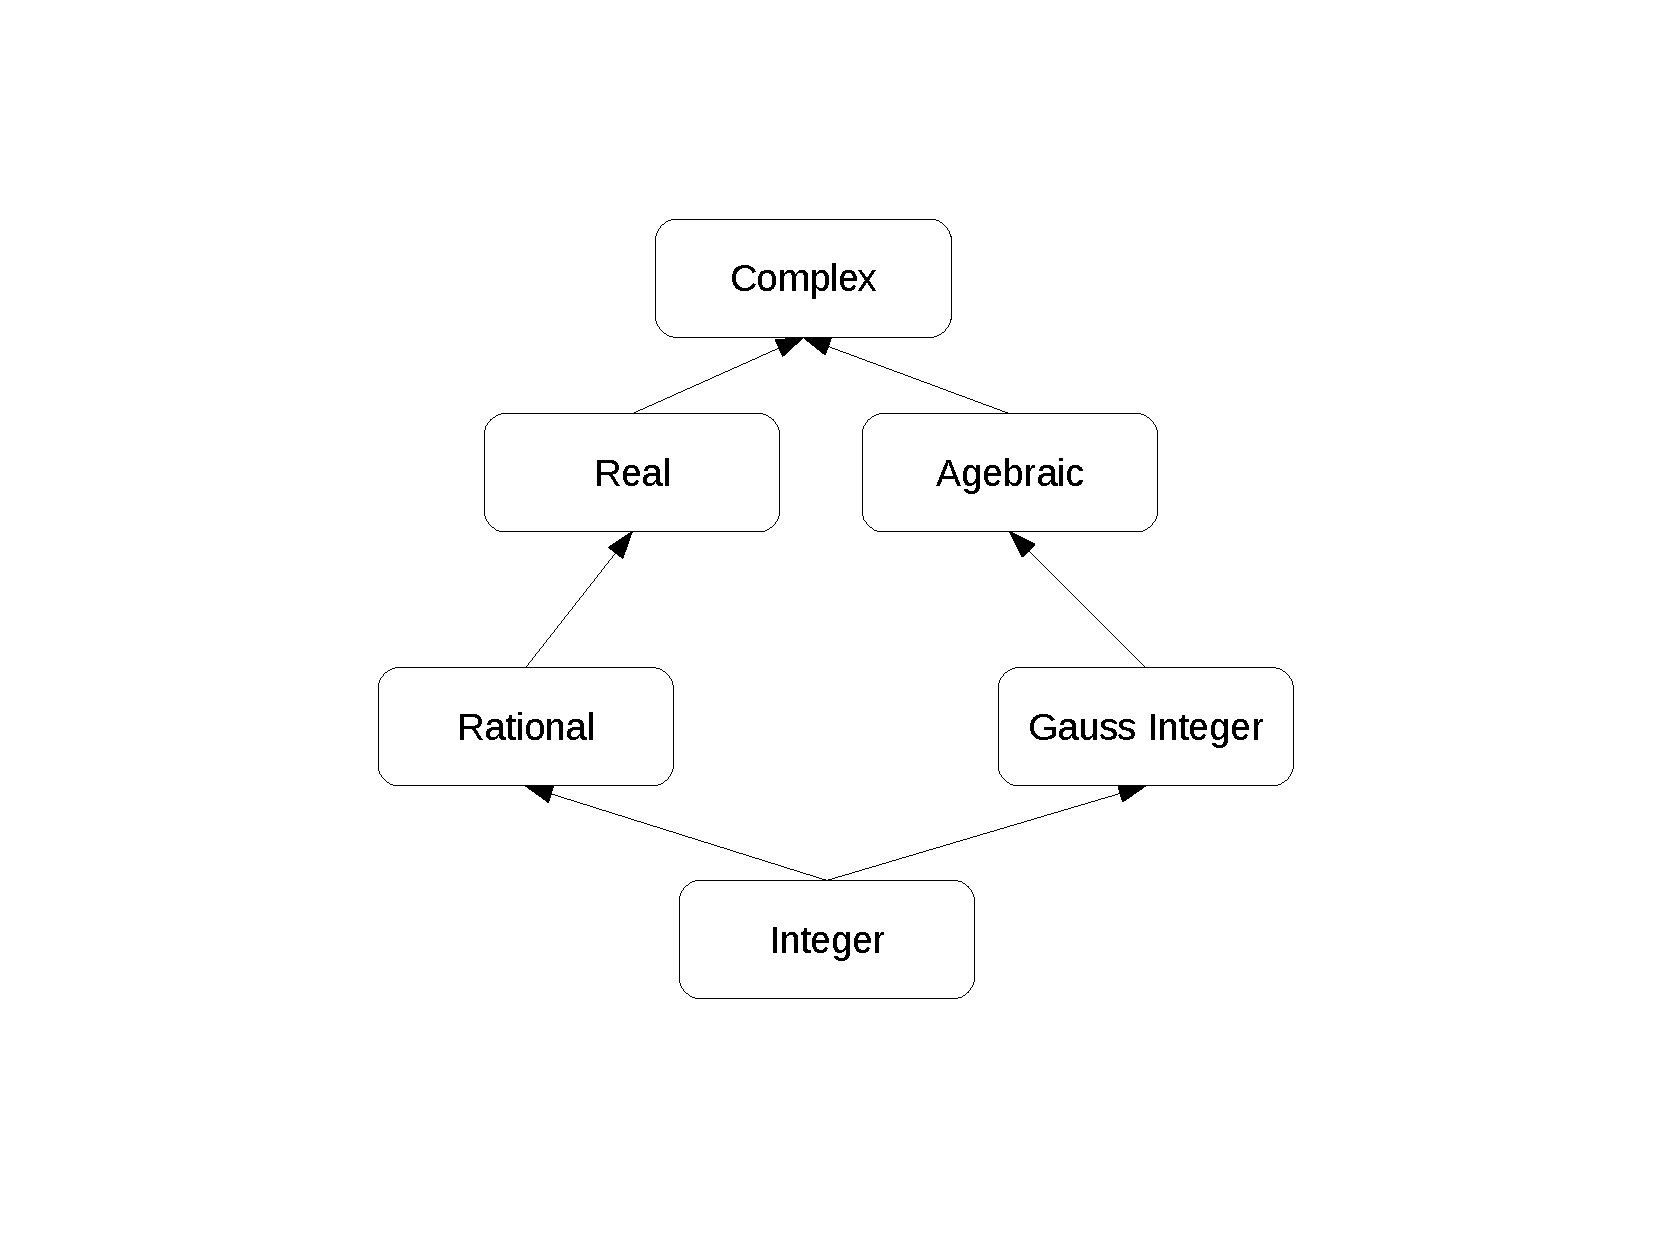
\includegraphics[scale = 0.3]{ExOntology.pdf}
  \caption{Ontology over numbers}
\end{figure}


This kind of structure is already available on a YAGO software (Yet An Other Great Ontology). However, this ontology is made from Wikipedia, but does not ensure the existence of an onto mapping from the set of articles of Wikipedia into YAGO.\\
The idea here is to use the wish of \textit{John} (specific or general) in order to construct an ontology over the articles he already read. Indeed, the goal will be to classify the articles among the partial order : \textit{"is more general than"}.To properly construct our structure, we have to ensure that articles proposed to \textit{John} avoid a cycle. Thus our recommander system will have to follow the property : 

\begin{pro}
The relation \textit{"is more general than"} induced by the constructed ontology is transitive. 
\end{pro}

This would ensure to have no cycle. The aim of the system is to construct a relation which is the nearest possible as \textit{"is more general than"}, using the wish of the user. More precisely, our ontology will be a \textbf{forest}.\\

Now that we have in mind the definition of ontology, let's try to find a way of using it to select articles. Let's remind that the user gave us a wish for the following article, either specific or general. If $wish = general$ then we will want to pick articles that are above (more general) our current article in the ontology, else (i.e $wish=specific$ ) we will pick articles under the current one. We will pick these articles as followed :

\begin{algorithm}
  \caption{Calculate $A^*$ the selected articles}
  \begin{algorithmic}
    \REQUIRE $wish \in \{specific , general\}$ , $N \in \mathbb{N}$ , $a_c \in A$, $\mathbb{O}$ ontology
    \STATE $A^* \leftarrow \emptyset$
    \WHILE {$ Card(A^*) \leq N $}
    \IF {$wish = specific$}
    \STATE $a_l \leftarrow $random leaf of $a_c$ in $\mathbb{O}$
    \STATE $a \leftarrow$ random article such that $(a,a_l) \in Edge(\mathbb{O})$ and $a \notin A_{visited}$
    \STATE $ A^*  \leftarrow A^* \cup \{a\}$
    \ELSE 
    \STATE $ r \leftarrow geometric.random(0.5)$
    \STATE $a_f \leftarrow $ random ancestor of depth $r+1$ from $a_c$
    \STATE $a \leftarrow $ random article such that $(a,a_f) \in Edge(\mathbb{O})$ and $a \notin A_{visited}$
    \STATE $ A^*  \leftarrow A^* \cup \{a\}$ 
    \ENDIF
    \ENDWHILE
    \RETURN $A^*$
  \end{algorithmic}
\end{algorithm}

\newpage


Here, $A_{visited}$ is the set of articles already visited : they are the nodes of $\mathbb{O}$ and $A$ the set of articles in Wikipedia in the selected language.\\\\
In this algorithm, when we ``Look for a random ancestor of depth $r+1$ from $a_c$'', it means that we pick a random article in the ontology already constructed $\mathbb{O}$ that follows a random walk of length $r+1$ begining on the state $a_c$.Like $\mathbb{O}$ is assumed to be a \textbf{forest}, these calls makes sense. 
\begin{rem}
  $r$ follows a geometrical law of parameter 0.5 because we want to be close to our current article in most of the cases.\\
\end{rem}
\textbf{Random pick}
\begin{itemize}
\item Articles are picked randomly in the page of an ancestor. However, most of these links are generally poor of interest. A way to avoid them will be described in the \textbf{implementation}.
\item Also, to take advantage of the wish of \textit{John}, we also may assume that in a Wikipedia page, general links are more likely to be in the introduction whereas specific (in reference to the current one) one are in the body. The choice of the article in both cases may follow this assumption to be more accurate.  
\end{itemize}

We then modify the ontology depending on the choice of the neural network and \textit{John}: 

\begin{algorithm}
	\caption{Actualize $\mathbb{O}$}
	\begin{algorithmic}
		\REQUIRE $\mathbb{O} \: previous \: ontology$, $A^* \: selected \: articles$
		\STATE $a\leftarrow NNcall(A^*)$
		\STATE Add the leaf $a$ in $\mathbb{O}$, attached to the article it was linked to
	\end{algorithmic}
\end{algorithm}
		
The new problem here is the lack of serendipity in our model. 

\subsubsection{The serendipity in the ontology}

In the previous algorithm, the set of candidate articles was chosen among the nearest neighbors in the constructed ontology.
In order to recommand to the user articles far from its habits, we present here another way to find articles, depending on the 'serendipity' factor I.\\
This algorithm presented below is an adaptation of the one above, which takes in account the serendipity factor, defined previously by the user thanks to the cursor serendipity bar. \\
Here is an algorithm which will select a article by serendipity, according to the importance given to it by \textit{John}. In that case, the wish (particular or general) is forgotten : it aims to get an article with no relation. 

\begin{algorithm}
  \caption{Calculate $A^*$ the selected articles}
  \begin{algorithmic}
    \REQUIRE $N \in \mathbb{N}$, $c \in \mathbb{N}$, $a_c\in A$
    \STATE $A^* \leftarrow \emptyset$
    \WHILE {$Card(A^*)\leq N$}
    \STATE Pick a random root of $\mathbb{O}$, $a_R$
    \STATE $a \leftarrow rand.article(A\setminus A_{visited})$
    \WHILE {$S_W(a_R,a)\notin I$}
    \STATE $a 
    \leftarrow rand.article(A\setminus A_{visited})$
    \ENDWHILE
    \STATE $ A^* \leftarrow A^* \cup {\{a}\}$
    \ENDWHILE
    \RETURN $A^*$
  \end{algorithmic}
\end{algorithm}

We pick random articles which match with a root of the ontology, but not too much, in order to keep the serendipity. The cursor bar influence the value of $I$, which must contain $0$ and such that the bound is well defined. This have to be studied in practice. According to $S_W$, and that the cursor of the bar is in $0,1$, $I=[0,\frac{1}{2}c]$ where $c$ is the cursor may be a good value (cf the tests of the similarity).\\
The value $0$ is kept because the neural network will take the nicest link and return it to John.\\\\

\textbf{Random pick}\\
In order to be more deterministic and accurate, we chose articles by popularity instead of randomness : popular articles will thus serves as a 'base' of articles, and the 'wish' of \textit{John} will help to propose him more specific and maybe unpopular ones.\\


The actualization of the ontology now create a new root, because \textit{John} has chosen an article which cannot be compared with another one, a priori. 
\begin{algorithm}[h!]
	\caption{Actualize $\mathbb{O}$ for serendipity}
	\begin{algorithmic}
		\REQUIRE $\mathbb{O} \: previous \: ontology$, $A^* \: selected \: articles$
		\STATE $a\leftarrow NNcall(A^*)$
		\STATE Create a new root in $\mathbb{O}$
	\end{algorithmic}
\end{algorithm}

By these two constructions on $\mathbb{O}$, the two cases ensures that at any time $\mathbb{O}$ is indeed a forest. \\\\

\begin{rem}[Cold start]
Here, the cold start is problematic because at the beginning we have no idea about the preferences of \textit{John}. In a first time, we will then propose him random articles, and more precisely articles among the most popular ones. 
\end{rem}


\section{Candidate Ranking}

\subsection{possible input in neural network}

\subsubsection{Category vector}

One of the very accessible tool to analyze a wikipedia page is(, as we mentioned ?), the use of the categories assigned to each page that can be obtained through the Wikipedia API.
Only looking at some often viewed wikipedia page, would have us thinking that those categories can act as key word for the article. For example the Michael Jackson wikipedia page has almost a hundred categories, quite diverse :
 \begin{center}
	\texttt{"21st-century American singers" "Accidental deaths in California" "African-American choreographers" "African-American rock singers" "African-American songwriters"  "People acquitted of sex crimes"}
 \end{center}

Nevertheless you would also notice that they are some less relevant categories. The first categories regard the page itself, it's link, it's sources, or even some precise month since it needs clarification.

 \begin{center}
	\texttt{"All articles with dead external links" "CS1 Spanish-language sources (es)" "Articles with dead external links from July 2013" "Wikipedia articles needing clarification from January 2017"}
 \end{center}
But an issue with this strategy may be that some very specific article won't be descripte precisly enough with there category 


Categories of the wikipedia page "functors" (in theory of category)
"Pages using web citations with no URL","Functors","Mathematics navigational boxes"

\subsubsection{Word2Vect and Wikidata}

\subsection{Wide and deep Neural Network}
\subsubsection{Wide : memorization/focus}
\subsubsection{Deep : generalization/serendipity}


\newpage

\section{System architecture}

First, we give a global diagram to expose interactions between the user interface, \textit{Wikipedia} pages, modules and \textit{Wikipedia} APIs. 

\begin{figure}[h!]
	\centering
    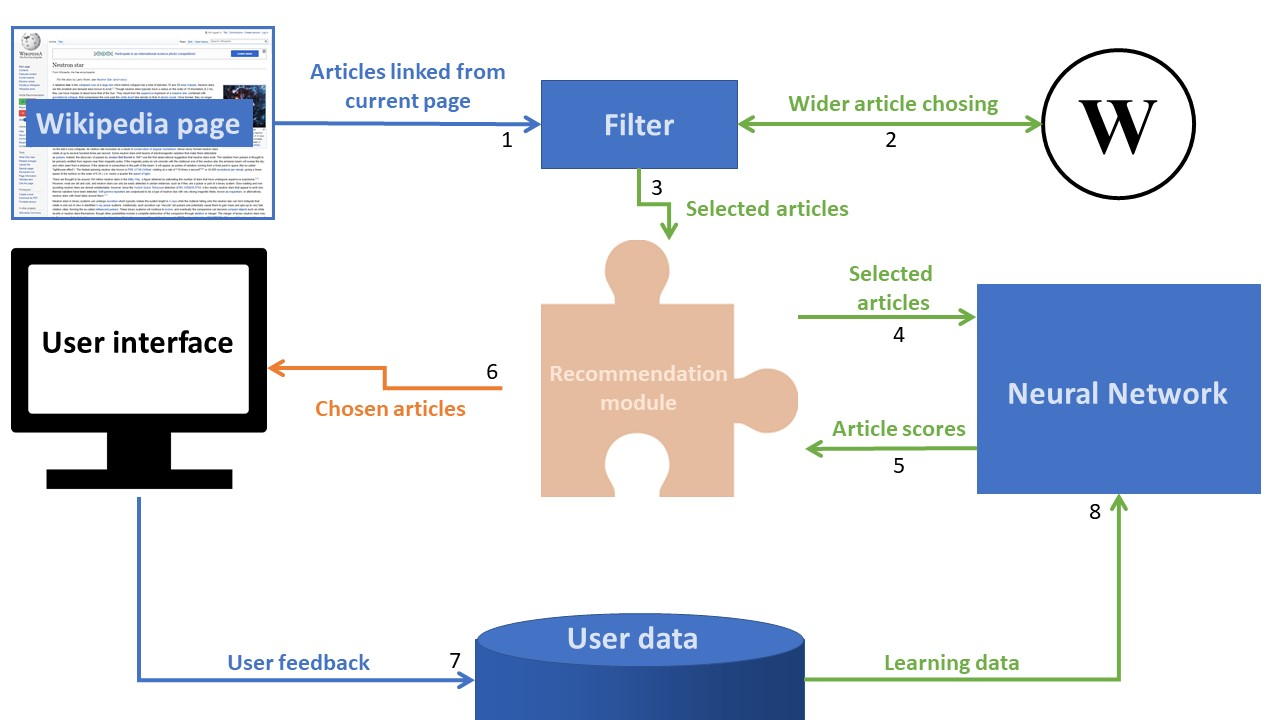
\includegraphics[width=400pt]{diagram.png}
    \caption{Global software's structure}
    \label{arch_glo}
\end{figure}

Blue arrows represent system's input, orange arrow is for the output. Green arrows explains how data is exchanged internally between the different modules. Arrowed labeling is defined as follows :
\begin{itemize}
\item \textbf{1)} \textit{Extraction of all links mentioned in the article (without the links of header, side, and footer)}.
\item \textbf{2)} \textit{Visit of article neighborhood (it may be 2-hop neighboring) to enhance serendipity, selection of best neighbors based on general criteria}.
\item \textbf{3)} \textit{Selected articles are injected into the recommendation module}.
\item \textbf{4), 5)} \textit{Recommendation module feeds the user-specific neural network with selected articles to sort them}.
\item \textbf{6)} \textit{Best articles are re-injected into the page, to be recommended to the user}.
\item \textbf{7)} \textit{User gives its feedback on proposed articles, reactions are stored locally}.
\item \textbf{8)} \textit{Thanks to user feedback, network structure is updated to fit user's interests}.
\end{itemize}

\subsection{Zoom on recommendation method}

\begin{figure}[h!]
	\centering
    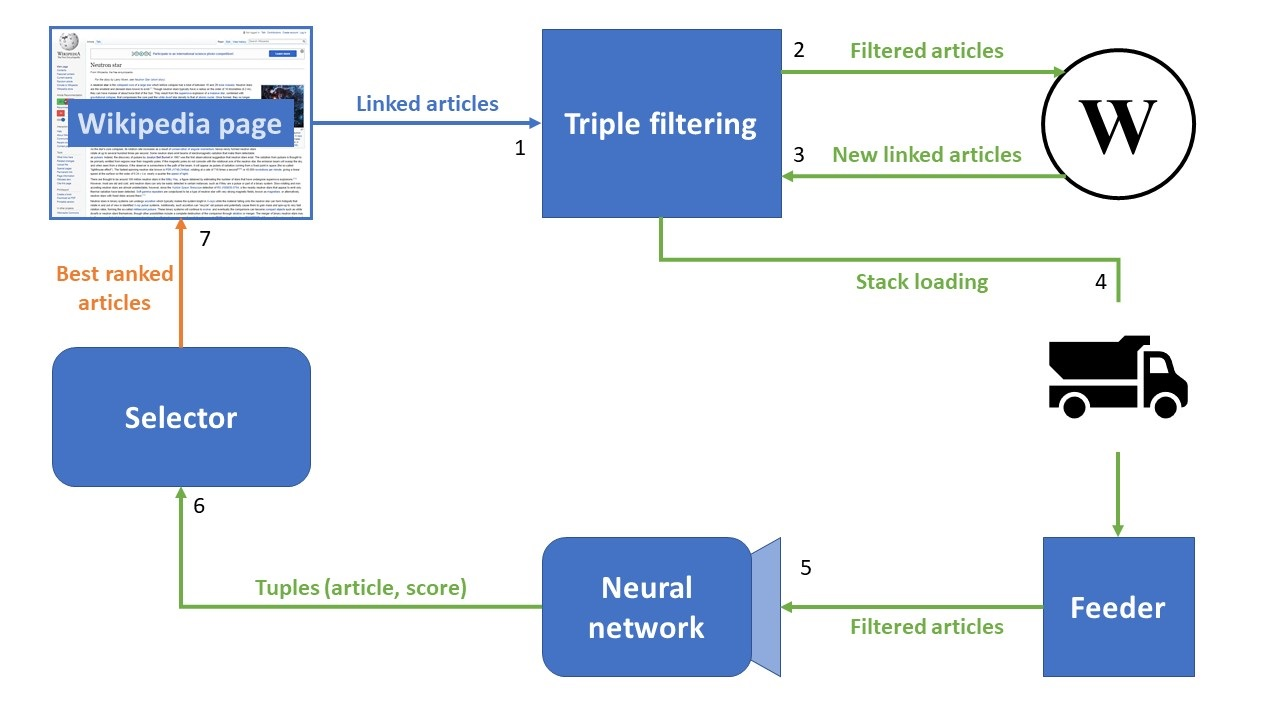
\includegraphics[width=400pt]{diagram_zoom.png}
    \caption{How recommendation method works}
    \label{arch_glo}
\end{figure}

\subsubsection{Triple filtering}

The main challenge which has been to be faced is the HTTP requests' efficiency problem. Indeed, the first idea is to get all page links, visit them all and sort them using some pertinence criteria. It was nevertheless technically impossible ; due to the size of HTTP requests, even performed asynchronously, the answer time was huge. \\

The solution developed was to introduce a triple filtering, which consists in three passes going more and more complex and time-expensive, but on less and less entries. It allowed the module to be able to explore pages to \textit{2-hops} from the original page

\begin{itemize}
\item \textit{Title-based filtering} With syntactically simple regular expressions, we can describe the set of hyper links that must be irrelevant. For instance there are years, ISBN codes, image links... All of them can be thrown away without even accessing their HTTP content.
\item \textit{Popularity-based filtering} In a second time, a probabilistic model has been introduced whose the purpose has been to determine how likely a page was to be liked by the user. \textit{Wikipedia}, through its \textit{API} called \textit{Wikimedia} allows, with a simple HTTP request weighting only a few dozens of characters, to access the views count of a certain page for a certain time lapse. Using it, one can identify connected trending content the user must be interested in.
\item {Content-based filtering} Finally, the module does its last selection by focusing on articles content. This part is the most expensive, as it is necessary to get the full page content for each remaining article, and to analyze it. This time, one focus on incomplete articles or poorly written (articles containing only a few words for example). \textit{This part could clearly be improved by a deeper text analysis, and probably get way better results.}
\end{itemize}

\subsubsection{Feeder and selector}

Feeder and selector manage neural network's input and output. Feeder gathers last filter output, then vectorizes it by applying the following operation ; 

\subsubsection{Neural network and learning}

\subsection{User interface}
We started the implementation of an in-browser plugin for Wikipedia suggestion.
The goal of this plugin is to insert an interface in any Wikipedia page that allows the user to give his opinion about this page. The plugin will keep an user profile up to date and suggest Wikipedia pages to the user that it considers relevant for this user.

As our goal is to introduce serendipity in such a system, we also added a cursor to parametrize a level of serendipity. Bigger this parameter is set, the less the user will be suggested pages about a topic he already eared of.

\subsection{Wikipedia API's}
% a few words about what both api provide


\section{Experimentation}
\subsection{Similarity}
Using Wikipedia official api, we were able to calculate the naive similarity between two pages defined at \ref{definition:S_w}. For example, the following code will prompt $0.6364$, the similarity processed between the page about Jimi Hendrix (of id 16095) and Michael Jackson (of id 14995351).
  \mint{javascript}|apiMod.distance(16095, 14995351, console.log); // "similarity(Michael J.,  Jimi H.)"|
  
Thus, we were able to experiment this distance over a set of web pages. We can thus qualitatively test this algorithm. It is not really hard to get examples where this calculation is irrelevant (for example, Michael Jackson is closer to France than Paris, cf. Figure \ref{fig:similarity}), but still, on many examples, it gives a trend that fits with the intuition.

\subsection{Using word2vec}


\begin{figure}[hb]
    \caption{Comparison of some pages of Wikipedia (cf. definition \ref{definition:S_w})}
    \label{fig:similarity}
	\centering
	\begin{tabular}{c|c|c}
		Page 1			&	Page 2			&	Similarity \\
		\hline\hline
		Michael Jackson	&	Jimi Hendrix	&	0.6364	\\
		Michael Jackson	&	France			&	0.8600	\\
		Paris			&	France			&	0.6842	\\
		Luxembourg		&	France			&	0.5416	\\
  \end{tabular}
\end{figure}


\section{Related Work}
%Recommendation systems
Recently, recommending web objects such as videos or news involved more research, like Youtube, Yahoo! News for instance. Based on literature content, recommendation systems can be roughly divided in two parts: content-based filtering and collaborating filtering approaches.\\
\textbf{Collaborative: }\\
The collaborative approach aims to find similarities between the user profiles. Users with similar preferences will be grouped and share their information. Then a single user's recommendations will be based on the information existing inside the group.\\
\textbf{Content-based: }\\ 
It consist on sequentially find content using past data items as an user's profile. Thus the goal is to find similarities between what an user liked and new items to recommend. It implies to have a good representation of items and good criteria to traduce an user's references. In general, data is represented using a vector space model.\\
Some systems use both content-based and collaborative filtering to try to avoid the drawbacks of each approach. We only use the content-based approach. Thus we need to evaluate the relatedness between two articles, which is a kind of distance, and use properly the user's feedbacks.\\
To determine which articles we propose, we use two kinds of neural networks.Deep neural networks (DNN) were first used for speech recognition and are now currently used to solve problems like picture recognition or classification in general. We use this type of neural network as well as a wide neural network in the filtering step to rank candidates.

\bibliography{scibib}

\bibliographystyle{Science}

\end{document}
